\chapter{Simulation Environment}\label{simulation}
    
    One of the main goals of this project is to study the performance of an urban mobile air quality monitoring system leveraging public transport vehicles, and the effects of various parameters including number of roadside access points, storage capacity (queue size) on mobile sensor platforms. Due to various reasons, working with actual buses proved to be impossible and so the decision was made to make simulation the mechanism through which the performance of this model would be evaluated. 

    In the model the buses would communicate with open WiFi access points as they move around the city, uploading the data they record to a central server. In order to model these buses as accurately as possible we required data about existing buses. Initially an attempt was made to use the Lothian Buses API, which can be seen in action at the website: \href{http://www.mybustracker.co.uk/}{\nolinkurl{http://www.mybustracker.co.uk/}}. However, due to the lack of position information this approach was quickly discarded. Talks with Lothian Buses gave access to 24 hours worth of position data of their ``liveried'' fleet. These are the buses which have route specific colouring and graphics and as such the buses will stick to a single route. This gave us a total of 145 different buses. It has been shown that by carefully selecting the routes of the buses we can achieve greater coverage~\cite{opensenserouteselection}, however this was not an option in this project. The coverage through these 145 buses, which cover 11 routes, is fortunately rather complete, with very few areas of the city being unvisited. This coverage map can be seen in figure~\ref{fig:route_coverage_map_liveried}, and can be compared to the map of all routes in figure~\ref{fig:lothian_bus_routes}.

    \centerimagewide{./images/Lothian_Bus_My_Routes_Coverage.png}{Edinburgh coverage across Lothian Buses routes with liveried fleet. This image comes from the Lothian Buses website and uses \emph{Google Maps}.}{fig:route_coverage_map_liveried}


    The data provided by Lothian Buses gives the position of the buses every 30 seconds and so in order to more realistically simulate the movement of the buses, the position between two readings was calculated using linear interpolation. The interpolation can cause some deviation from the correct path around corners, however, due to the fact that buses in Edinburgh can travel no faster than 30mph, which is approximately 13.4m/s, the buses can travel at most 402m between readings. This will only happen should the bus be travelling in a straight line at this maximum speed. By adding in a corner, which is where we would see deviation from the actual path, we can be at most 142m, proven via trigonometry, from the true position. The chances of this happening are extremely low however and it is likely that we will be much closer. This error, while potentially lowering the efficiency of our algorithm slightly, is unlikely to have a large effect. An area of future work would be the improvement of the interpolation algorithm. By using a slightly more advanced algorithm, such as one of the ones seen in section~\ref{background_interpolation_methods}, we could potentially achieve a more accurate simulation. A different alternative would be to use a route calculation API of some kind, such that the route by road could be calculated between two points. 

    With regards to the data for the wireless points, this data was provided by PhD student Arsham Farshad, who travelled around Edinburgh on various buses, recording the locations of wireless access points, their relative signal strengths, and more importantly, those which are open. From the initial choice of roughly 2,000 open WiFi APs, the 82 with the strongest signal, when measured from a bus, were chosen. As will be seen in section~\ref{simulation_simulator_options_simulation_speed_optimisation}, the processing time of the simulation is heavily dependent on the number of APs. Due to this no simulation is run with more than 50 APs. 


    In simulating a complex model like this, certain questions need to be answered and challenges overcome. This section answers these questions, such as the decision of which simulator to use, and how to use it as efficiently as possible. 

    \section{Simulator Choice}\label{simulation_simulator_options_simulator_choice}

        The initial simulator choice of \emph{NS-3} was recommend by Dr. Marina. NS-3 was recommended due to its reputation for being extremely powerful and realistic. This reputation has caused NS-3 to be used in various projects and experiments with great success~\cite{highperformancesimulatorofadhocnetworks}.  Furthermore, when compared with other well known network simulators, such as NS-2, Omnet++ and JiST, it performed the best overall~\cite{networksimulatorcomparison}. 

        Initial simulation tests were completed with NS-3, however after 4 weeks of testing it became clear that the learning curve of NS-3 was significant, and was in danger of delaying the progress of the entire project. Due to this danger other simulators were explored. 

        Omnet++ (\emph{Objective Modular Network Testbed in C++}) was the suggestion of Professor Arvind and Dr. Viglas who have supervised students using this simulator. Research into the simulator showed that Omnet++ is not a network simulator in the same way that NS-3 is. Instead, it is a framework which uses discrete events as its basis. Simulations for Omnet++ are also written in C++, but follow a different approach. The simulator uses a collection of modules which follow a strict object oriented model. New modules can be created by sub-classing others, or simply connecting them together into a greater module. With respect to these modules, there are many different collections of these modules, known as ``models''. Many models exist for Omnet++ including, but not limited to, Castilla, INET and MiXiM, with the latter two being of particular interest. 

        MiXiM is used in Omnet++ for creating wireless networks with a particular focus on the lower layers of the network stack. The models provided in the MiXiM framework are extremely detailed and include radio wave propagation, interference estimation, radio transceiver power consumption and wireless MAC protocols~\cite{miximvision}. MiXiM has no support for the upper network layers and if you need these then you need to rely on another model such as INET, or create your own. 

        INET is so closely related to Omnet++ that it is rare to use Omnet++ without using INET. INET provides models for the internet stack, as well as wired and wireless link layer protocols. It also contains many different application layer models, mainly for demonstration purposes.  

        In terms of performance and accuracy, when using the INET and MiXiM models, Omnet++ rivals NS-3~\cite{networksimulatorcomparison}.


    \section{Data Collection}\label{simulation_simulator_options_data_collection}

        One of the further advantages of choosing Omnet++ was the built in sophisticated data logging framework. This framework made it extremely easy to record information about the simulations, such as packet loss, latency and throughput. However, after running a simple simulation with all 145 buses and 50 access points for a simulated time of 10,000 seconds, the output of this logging frame work was measured at over 40GB. Furthermore, it was not in an easily accessible format for further analysis using a scripting language. As such, the decision was made to create a custom logging framework which would reduce the size of these data files. Running the same simulation with the new framework reduced the file size to around 3GB, which when compressed came down to around 200MB. This huge space saving allowed for more simulations to be run as the data did not have to be collected at the end of each simulation to avoid running out of disk space. 

    \section{Simulation Speed Optimisation}\label{simulation_simulator_options_simulation_speed_optimisation}

        When the simulation was completed, multiple tests were run in order to profile the performance of the simulator and simulations. The results of this profiling can be seen in figure~\ref{fig:access_points_speed}. These results show that when there are no buses, the number of simulated events per second increases with the number of access points. The relationship appears to be linear in nature, however the most extreme data point indicates that it may be a polynomial or exponential relationship. The reasoning for this being that most access points are not in range of any others when we have a lower number of them and so they do not have any effect on each other. The number of events is correlated with the simulation time. That is, the more events there are per second, the longer it will take to simulate one second. The speed of a simulation is defined by the number of events per simulated second, as the number of events is the limiting factor in terms of physical processing. For example, a computer which can process 100,000 simulated events per actual second, can simulate a simulation which generates 10,000 events per simulated second 10 times faster than reality. 

        When we add in our buses we can see that things change dramatically. The number of events now increases exponentially with the number of access points. This has a similar effect on the total simulation time, causing it to also increase exponentially. 

        Due to these effects, we cannot feasibly run simulations with more than 50 access points. According to figure~\ref{fig:access_points_vs_time_and_events}, increasing to just 60 access points would almost double our total simulation time. 

        \begin{figure}
            \centering
            \begin{subfigure}{0.45\textwidth}
                \centering
                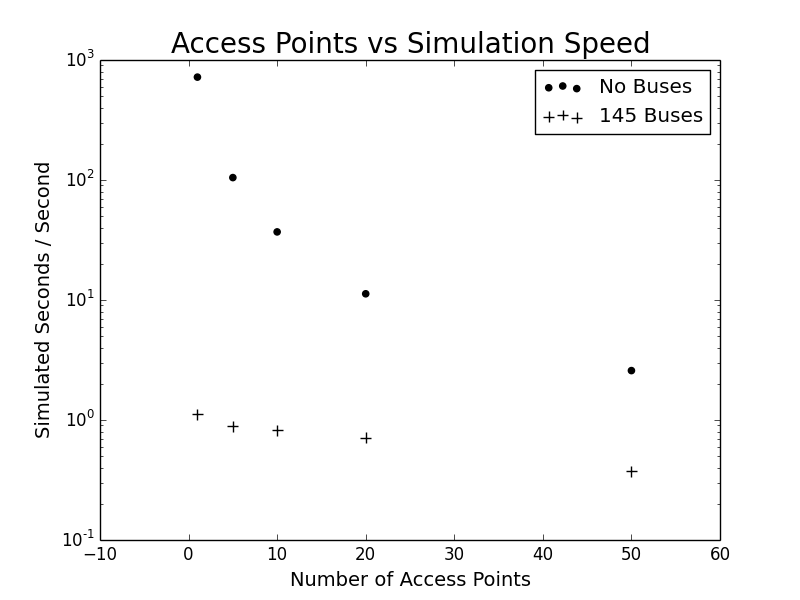
\includegraphics[width=\linewidth]{./images/AP_vs_Simulation_Speed.png}
                \caption{Simulation speed as a function of the number of access points.}
                \label{fig:access_points_speed}
            \end{subfigure}%HODOR
            \begin{subfigure}{0.45\textwidth}
                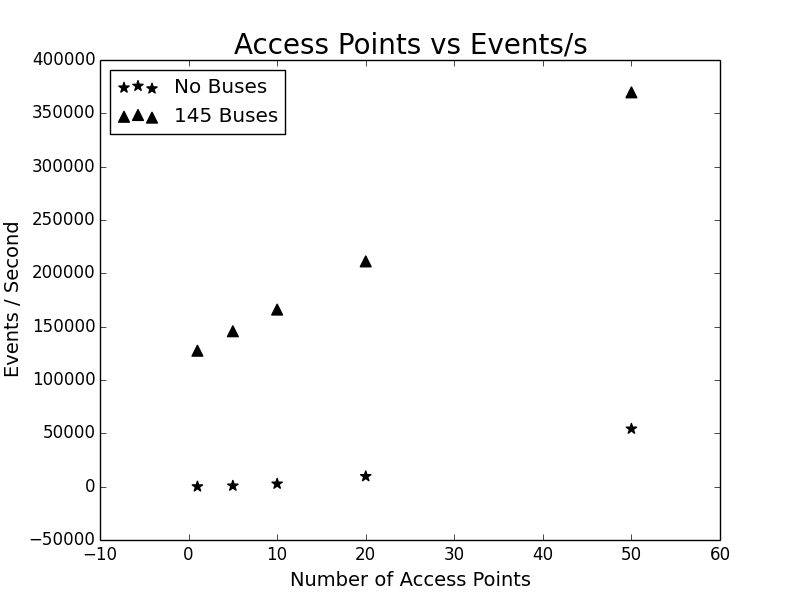
\includegraphics[width=\linewidth]{./images/AP_vs_Events.png}
                \caption{Number of events as a function of the number of access points.}
                \label{fig:access_points_events}
            \end{subfigure}
            \caption{Simulation speed and number of events as a function of the number of access points in the simulation. This has been performed for no buses and 145 buses in the simulation.}
            \label{fig:access_points_vs_time_and_events}
        \end{figure}

        When running a full simulation with 50 access points and all 145 buses it took approximately 3 days to simulate 1 day. In order to be able to perform all desired experiments and be able to repeat them multiple times in the 6 months which remained at this point, the simulation would have to be improved dramatically. Fortunately, Omnet++ provided a mechanism for this. 

        \emph{MPI}, which is an acronym for Message Passing Interface, is supported by Omnet++~\cite{omnetmpi}. MPI allows simulations to run on multiple cores concurrently. Ordinarily Omnet++ runs on a single core, however if it were to use MPI on a 4 core machine then theoretically it is possible to achieve a 4 fold performance increase. In practice the increase is lower due to the message passing overhead, but we would still hope to see the simulation time improve dramatically. The simulation configuration was set to allow MPI and some speed tests were run. The results of these tests showed that the simulation was almost twice as slow when using MPI. Further investigation revealed the cause of these problems. 

        
        \centerimage{0.4\textwidth}{./images/Bi-Partite_Network.png}{An example of a suitable place to partition a network, represented by the red line. }{fig:bipartite_network}

        MPI in Omnet++ works extremely well when the networks are cleanly partitioned. For instance, modelling two subnets connected by a switch. Figure~\ref{fig:bipartite_network} shows a logical point to partition a network with that setup. In this example, one subnet would run on one core, and the other on a separate core. All communication within the subnet would remain on that core, which would cause no additional overhead. Any communications between subnets would then use MPI. In our model we do not have any clean point to partition. With 145 buses moving around the city and 50 access points it would be difficult to devise an optimal partition. This problem could potentially be solved using machine learning, however that is beyond the scope of this project. It is theorised that if all entities, that is the buses and access points, were run on a separate core, perhaps using many machines, we may see a performance boost, however this was infeasible. 

        Due to parallelising a single simulation failing, a different approach was taken. Instead of running one simulation on $n$ cores, the decision was made to run $n$ simulations on $n$ cores, essentially one simulation per core. Initial testing was performed on a dual core machine with two simulations. The results showed that the simulations both took more than twice as long as the single test. When this was tested on a quad core machine however, the simulations took slightly less than double the time. This means that the total time to run both simulations was less than running each sequentially, which is a clear improvement. Unfortunately continuous access to this quad core machine was not available and an alternative had to be found. 

        Currently, popular methods of performing large scale computations are to use virtual machines hosted by a third party. Common companies to use for this are \emph{Amazon}, \emph{Rackspace} and \emph{Digital Ocean}. Based on the requirements above, the aim would be to choose multiple instances with 4 cores for the cheapest price. In terms of cost, Digital Ocean was a clear winner, however it was 4 times as expensive to get a 4 core machine as it was to get a 2 core machine. As such, simulations were run on 5 dual core machines. Each machine was given a different random sampling of access points, and all simulations on each machine were run sequentially. This reduced the run time of some tests from over a month to just under a week. 



